\section{Kravspecificering og Use cases}
I dette afsnit vil vi beskrive vores kravspecificering og vores Use cases, som vi har udarbejdet til denne rapport.
\subsection{Kravspecificering}
I dette afsnit har vi taget udgangspunkt i kundens vision. Vi har læst den igennen, og stillet spørgsmålstegn, ved de ting, der kunne være tvivl om. Kunden er dog blevet til kravspecificering i forløbet, og derfor var der få tvivlsspørgsmål.
\begin{enumerate}
\item Hvad skal der ske, hvis en spiller ikke kan betale det han skal?
\item Skal man betale, hvis man lander på et felt, der er ejet af en bankerot spiller?
\item Skal man have mulighed for at købe eet felt, der tidliger var ejet af en spiller, der nu er gået bankerot?
\end{enumerate}
Vores kontakt i firmaet, som er vores projektleder, har besvaret disse punkter på følgende måde
\begin{enumerate}
\item Spilleren der ikke kan betale, må betale det han har, og går herefter bankerot.
\item Feltet er ikke længere ejet af nogen, og derfor skal der heller ikke betales.
\item Da feltet ikke længere ejes, skal man kunne købe det.
\end{enumerate}
\subsection{Use Cases}
\todo[inline]{Thomas A: Indsæt tekst fra fully dresses og brief + diagram}
Vi vil i dette afsnit beskæftige os med 2 use cases, som er beskrevet i nedenstående diagram. Til vores spil har vi lavet en fully dressed use case, og til vores test har vi blot lavet en brief use case.
\subsubsection{Use Case Diagram}
\begin{figure}[ht]
\centering
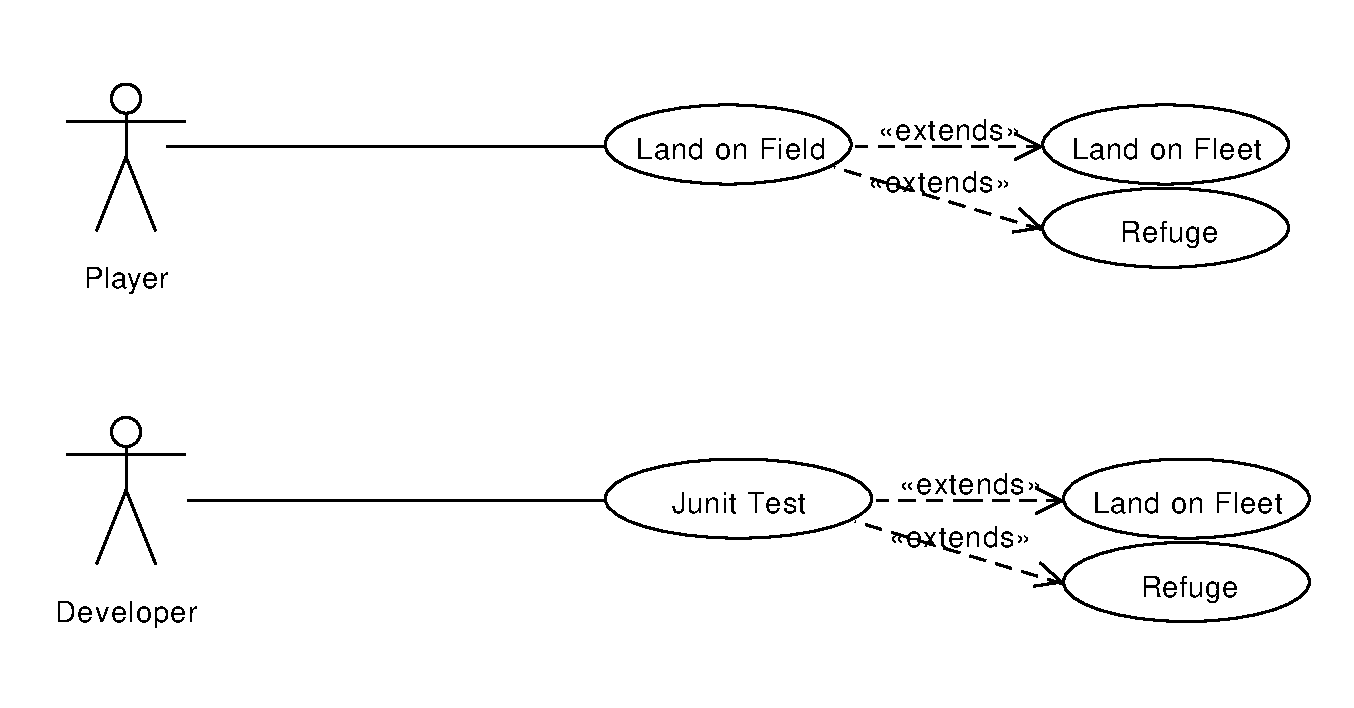
\includegraphics[width=1\textwidth]{UseCase.pdf}
\caption[<Text for the list of figures>]{Use Case Diagram}
\label{fig:figure 2}
\end{figure}
\newpage
\subsubsection{Fully Dressed Use Case}
Vi har i dette afsnit beskrevet vores use case med en fully dressed use case for spil.
\subsubsection*{Use Case}
Land on Field
\subsubsection*{Scope}
Spil
\subsubsection*{Level}
Bruger Konsekvens
\subsubsection*{Primary actor}
Spiller
\subsubsection*{Stakeholders and Interests}
Spiller: vil tjene penge og undgå falit
\subsubsection*{Preconditions}
Eclipse er installeret på maskinen.
\\
Programmet er kørende.
\subsubsection*{Main Success Scenarie:}
\begin{enumerate}
\item Spiller starter spillet
\item Spiller indtaster Navn
\item Spiller Ruller med terningerne
\item Spiller lander på et felt med positiv konsekvens
\item Spiller modtager penge
-- Spiller gentager punkt 3-5 indtil en spiller går falit
\item System checker for tabere
\item System viser vinder
\item System lukker ned
\end{enumerate}
\subsubsection*{Extensions Alternative scenarier:}
*a - til hvert et tidspunkt
\begin{enumerate}
\item Spiller lukker spillet ved at taste "q"
\end{enumerate}
4a. Spiller lander på et felt med negativ konsvens
\begin{enumerate}
\item Spiller betaler regning
\item Spiller kan betale regning --> punkt 6-8 i main success aktiveres
\end{enumerate}
4b. Spiller lander på et felt uden konsekvens
\begin{enumerate}
\item Spiller står uberørt af felt mht. pengebeholdning
\item Spiller bliver givet ekstra tur
\\
5a. Spiller skal betale penge
\item  Spiller betaler regning
\item  Spiller kan ikke betale  --> punkt 6-8 køres
\end{enumerate}
\subsubsection*{Specielle Krav:}
\begin{itemize}
\item Skal kunne køre på en Windows maskine med Java EE på DTU's computere
\item Skal kunne spilles af en almindelig bruger
\end{itemize}
\subsubsection{Brief Use Case af Tax}
Vi har valgt at lave en brief use case over vores tax.
\\

\textbf{Account Test}
Når en spiller lander på et tax felt, skal spilleren bestemme om han vil betale 4.000 eller om vedkommende vil betale 10 procent af deres formue. Valget afgør så hvor meget der skal betales. 